\chapter{Background}
\label{cha:background}
This chapter provides an overview of the text mining field along with previous work in the area and all necessary background information required to understand the major tasks involved in this project.

\section{Text Mining}
\label{sec:textmining}
``Text mining is the process of extracting interesting information and knowledge from unstructured text"\cite{hotho-etal-ldv-2005} and its applications tend to work in two steps, first using an Information Retrieval(IR) application to narrow the search space, and then they extract significant parts of the retrieved texts\cite{Polajnar2006}. This general process usually involves structuring a source text by means of parsing and other linguistic analysis, then finding patterns in this structured data and then interpreting this output. Text mining is fundamentally different from standard web searching in that web searches rely primarily on information that is already known. However, the goal of text mining is to discover interesting, previously unknown information\cite{Gupta_Lehal_2009}. 
%Its high-level subfunctions can be seen in Figure~\ref{fig:tm} and these will be further explored below.
\begin{figure}
\begin{center}
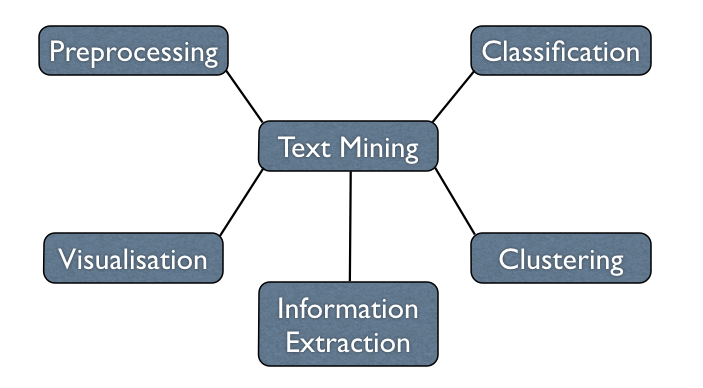
\includegraphics[width=10cm]{textmining}
\end{center}
\caption{Aspects of text mining}
\label{fig:tm}
\end{figure}


\subsection[Information Retrieval]{Information Retrieval(IR)}
IR is the process of retrieving textual documents which may contain the answers to questions but do not answer these themselves\cite{hotho-etal-ldv-2005}.


% MENTION MACHINE LEARNING V RULE/DICTIONARY BASED APPROACH
\subsection[Natural Language Processing]{Natural Language Processing(NLP)}
\subsubsection{Tokenisation}
\subsubsection{Part of Speech(POS)}
\subsubsection{Lemmatisation}
\subsubsection{Named Entity Recognition(NER)}




\section[Sentiment Analysis]{Sentiment Analysis and Opinion Mining}

\section{Twitter Mining}
There has been several previous works on text mining Twitter posts, however, the bulk of these have focussed solely on biomedicine and the financial sector.


% MOVE TWITTER API HERE? FROM IMPLEMENTATION CHAPTER
